
\documentclass{standalone}

\usepackage{tikz}
\usetikzlibrary{shapes.geometric}
\begin{document}
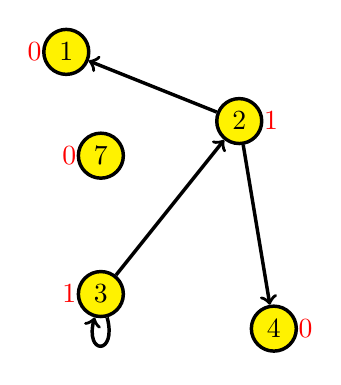
\begin{tikzpicture}
[every node/.style={inner sep=0pt}]
\node (2) [circle, minimum size=16.25pt, fill=yellow, line width=1.25pt, draw=black,label=right:$\color{red} 1$] at (100.0pt, -62.5pt) {\textcolor{black}{2}};
\node (4) [circle, minimum size=16.25pt, fill=yellow, line width=1.25pt, draw=black,label=right:$\color{red} 0$] at (112.5pt, -137.5pt) {\textcolor{black}{4}};
\node (1) [circle, minimum size=16.25pt, fill=yellow, line width=1.25pt, draw=black,label=left:$\color{red} 0$] at (37.5pt, -37.5pt) {\textcolor{black}{1}};
\node (3) [circle, minimum size=16.25pt, fill=yellow, line width=1.25pt, draw=black,label=left:$\color{red} 1$] at (50.0pt, -125.0pt) {\textcolor{black}{3}};
\node (7) [circle, minimum size=16.25pt, fill=yellow, line width=1.25pt, draw=black,label=left:$\color{red} 0$] at (50.0pt, -75.0pt) {\textcolor{black}{7}};
\draw [line width=1.25, ->, color=black] (2) to  (1);
\draw [line width=1.25, ->, color=black] (3) to  (2);
\draw [line width=1.25, ->, color=black, loop below] (3) to (3);
\draw [line width=1.25, ->, color=black] (2) to  (4);
\end{tikzpicture}
\end{document}
